\documentclass[../../../main]{subfiles}
\begin{document}

\section{方法}

\subsection{電磁石の磁場分布測定}
電磁石が発生する磁場の分布を測定する。
電磁石を上から見た図を図\ref{fig:electromagnet}に示す。
この電磁石に適当な励磁電流を流し、
$y$軸上を中心からポールピースの端まで$\SI{5}{\milli\meter}$ずつガウスメータを移動させながら磁場を測定する。
\begin{figure}
    \centering
    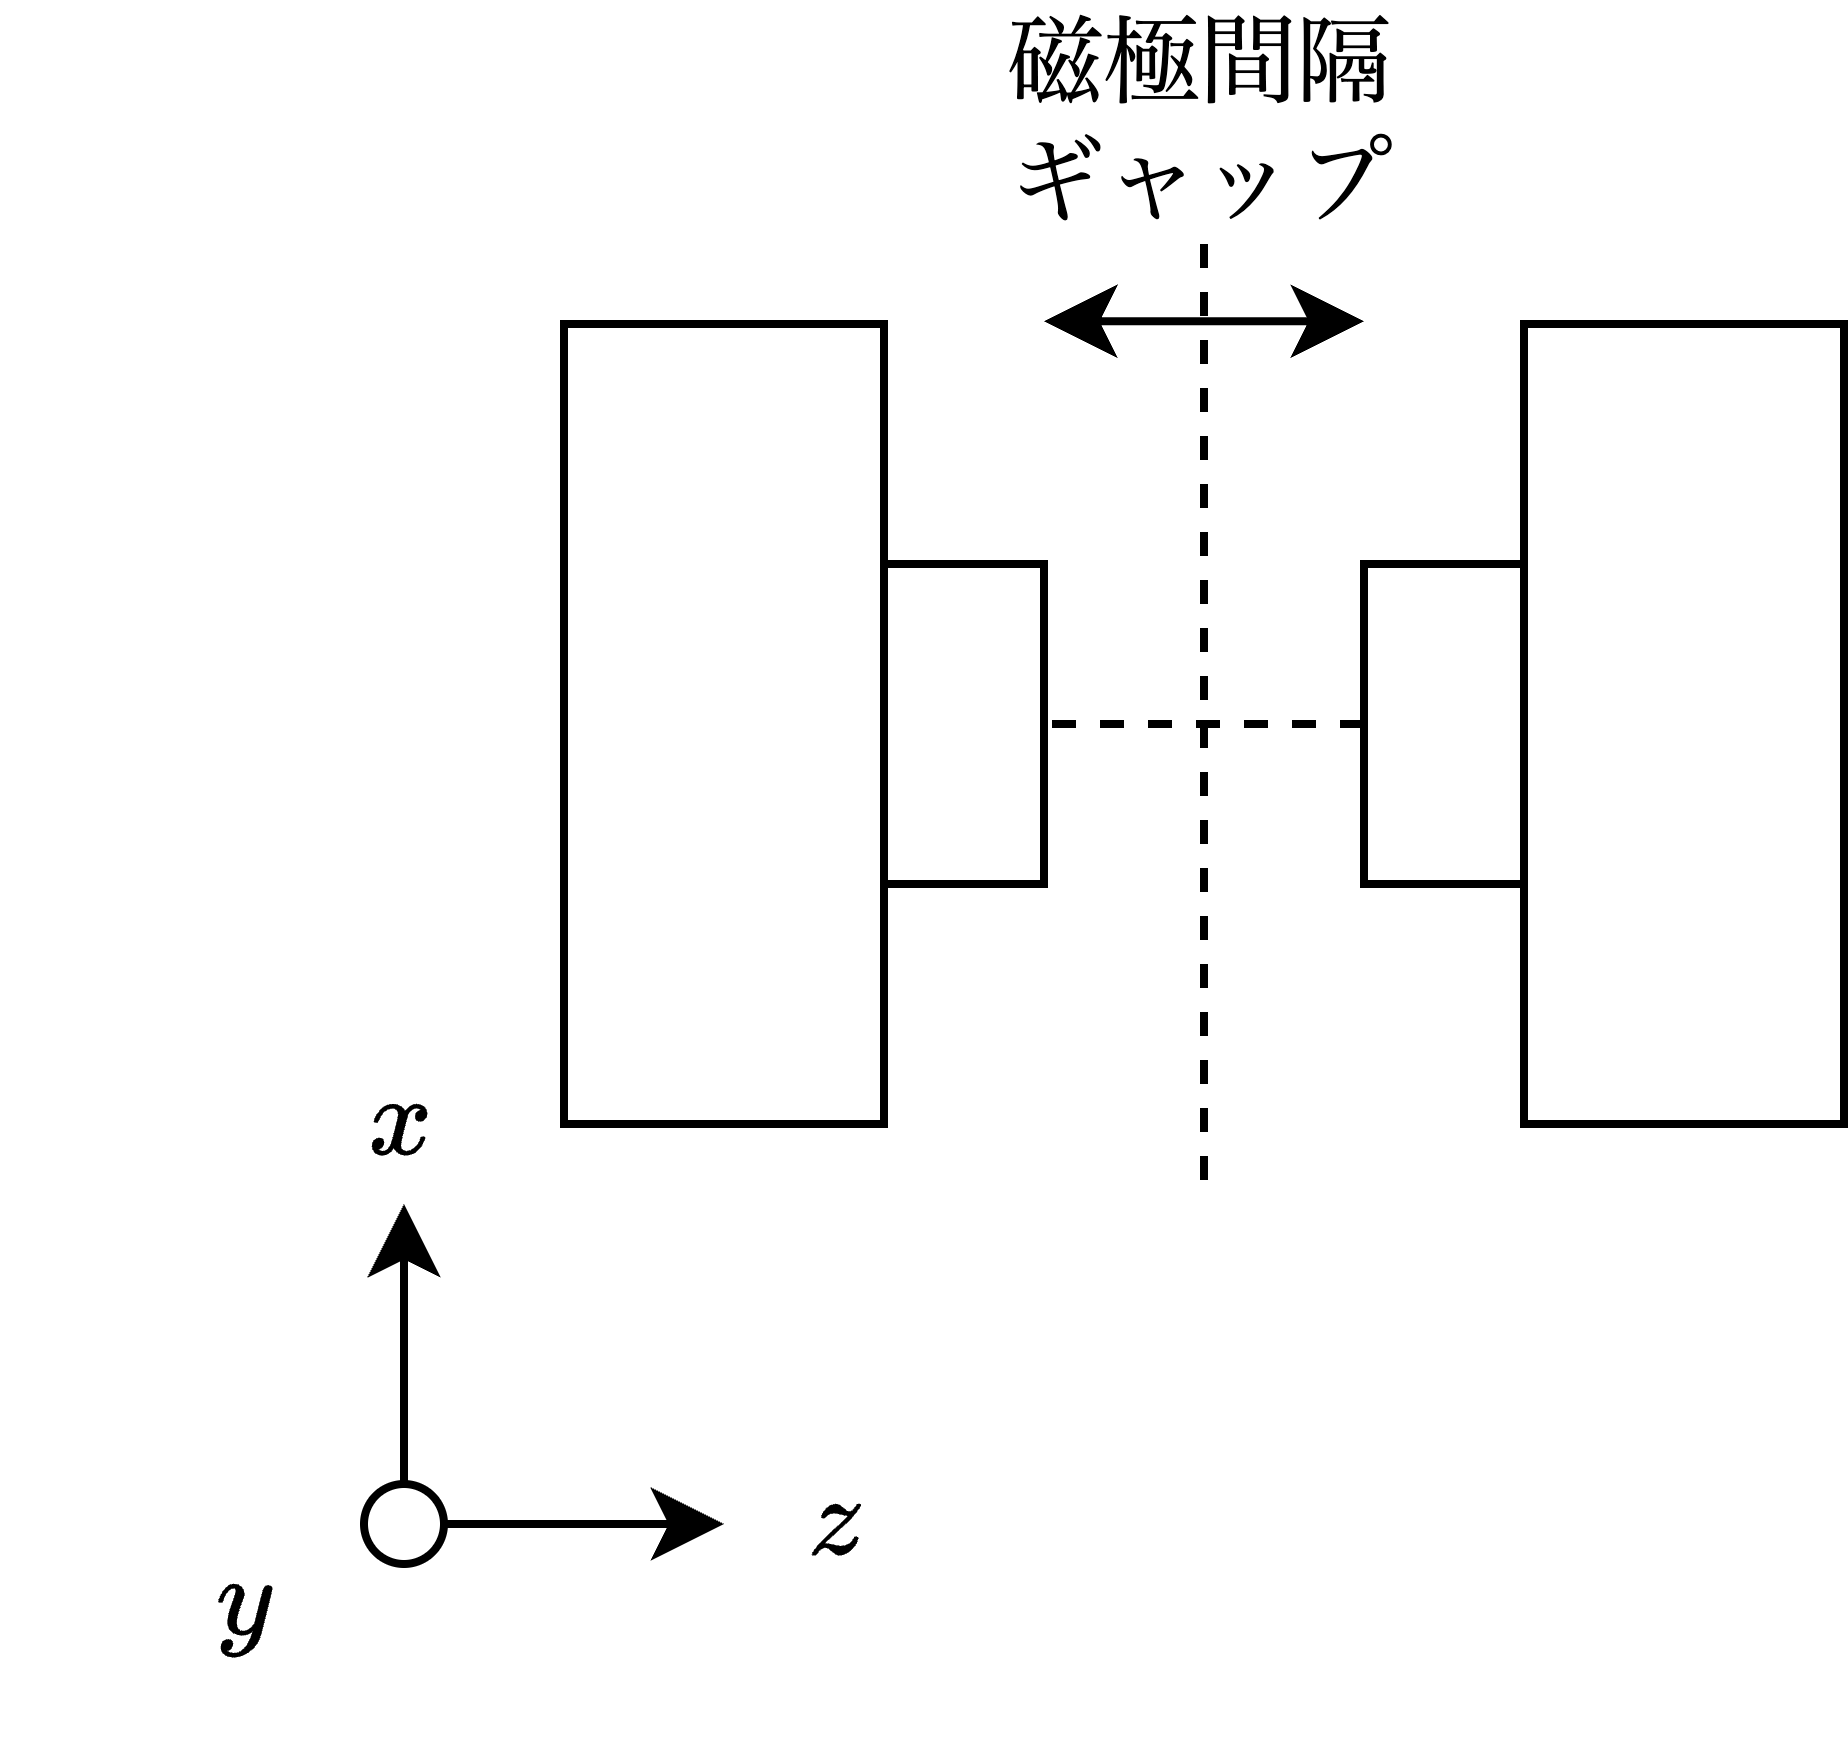
\includegraphics[width=0.5\linewidth]{src/figures/electromagnet/electromagnet.png}
    \caption{電磁石を上から見た図}\label{fig:electromagnet}
\end{figure}


\subsection{励磁電流と磁場の強さの測定}
電磁石に与える励磁電流とそれによって生じる磁場の強さの関係を測定する。
まず、ガウスメータのプローブをz軸に平行になるように設置し、
励磁電流を変化させ、そのときの磁場を測定する。
これによって調べた励磁電流による磁場の強さの変化の特性をもとに以後の実験を行う。

\subsection{励磁電流による電流の変化}\label{subsec:current}
実験装置の回路を\ref{fig:exp}に示す。
まず、$B_z$を変化させながら、$I_x$の向きと$V_H$を測定する。
次に、$I_x$をいくつかの値で設定し、そのときに$B_z$を変化させ$V_H$の変化を測定する。
$I_x$や$B_z$を逆向きにした場合も測定すること。
このデータおよび、\ref{eq:hall-voltage}、\ref{eq:hall-voltage}、\ref{eq:mobility}、\ref{eq:mobility-1}式などから
キャリアの種類、ホール係数、キャリア数密度を求める。

\subsection{半導体の電圧降下の測定}\label{subsec:resistance}
磁場がかかっていない状態で、半導体に電流$I_x$を流し、そのときの電圧降下$V_R$を測定する。
いくつかの$I_x$に対して$V_R$を測定し、次式から半導体の抵抗を求める。
\begin{equation}\label{eq:resistance}
	R = \frac{V_R}{I_x} = \rho \dfrac{l}{tw}
\end{equation}
さらに、\ref{eq:resistance}式から比例係数$\rho$を求める。
\begin{equation}\label{eq:resistance-coefficient}
	\rho = \dfrac{Rtw}{l}
\end{equation}

試料に磁場がかかっている場合も同様に$R$、$\rho$を求める。

\subsection{温度依存性}
試料の温度を\SI{50}{\celsius}、\SI{70}{\celsius}、\SI{100}{\celsius}にし
\ref{subsec:current}節、\ref{subsec:resistance}節の実験を行う。




\begin{figure}
	\centering
	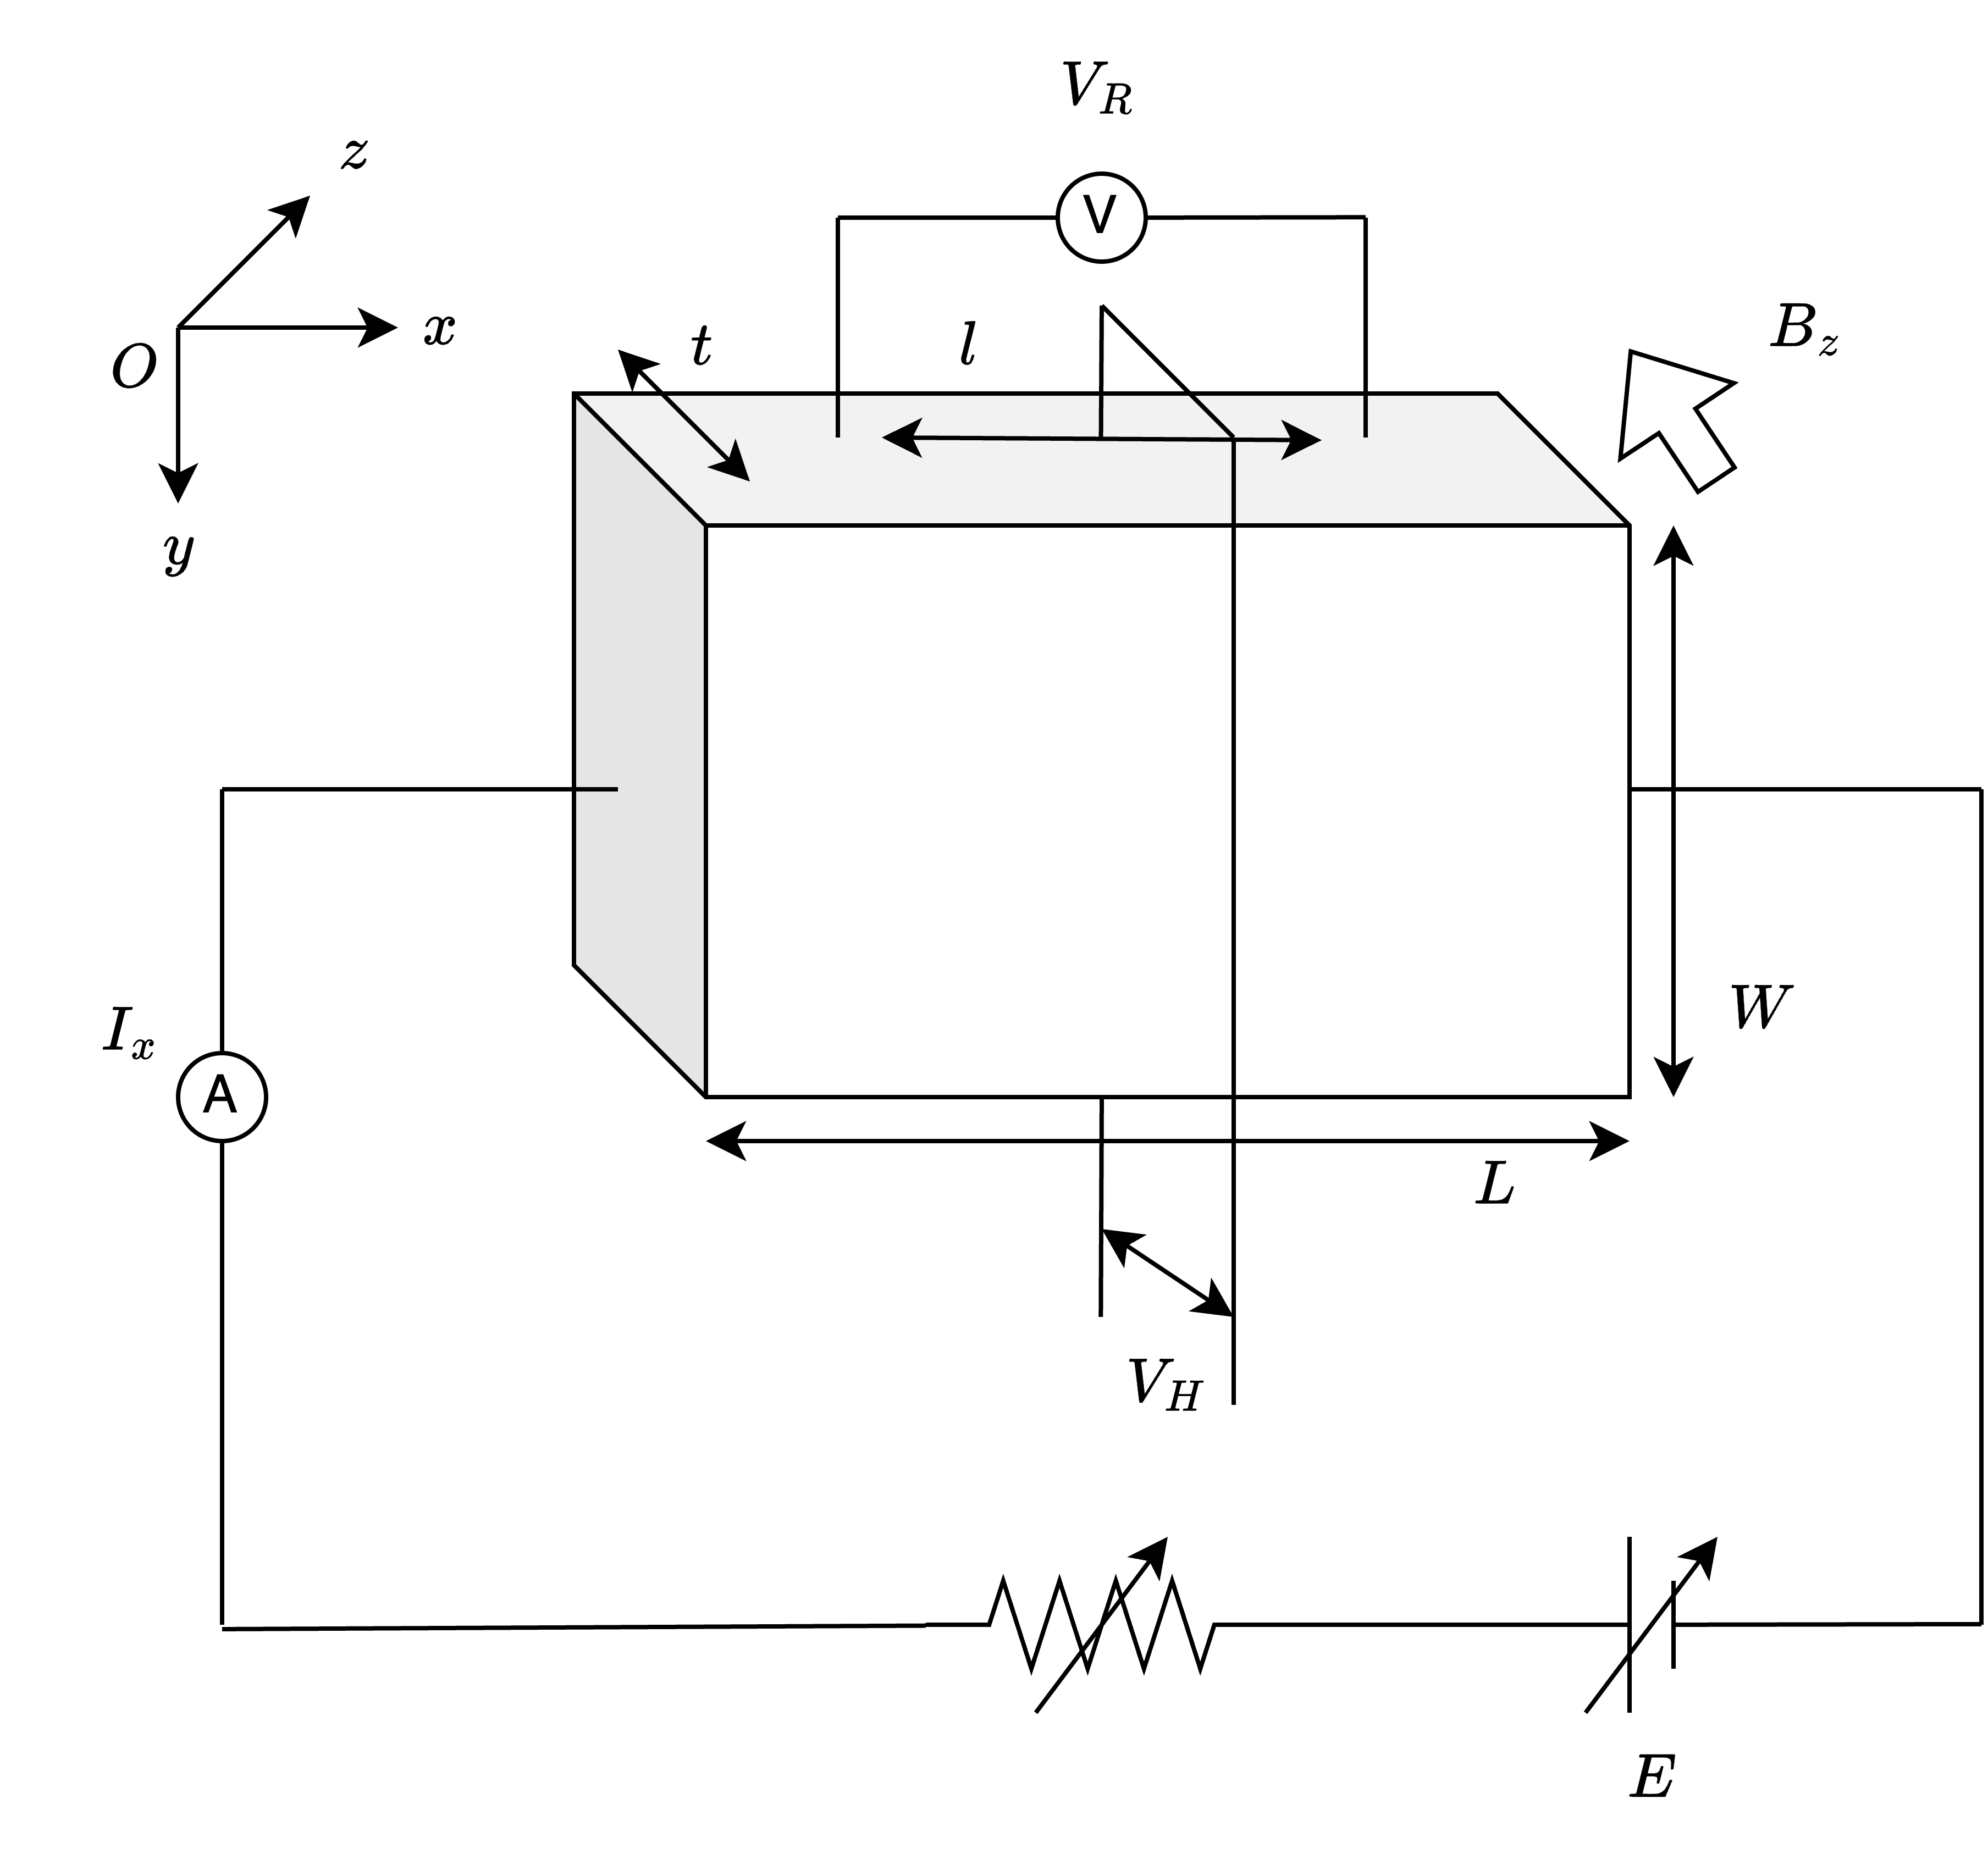
\includegraphics[width=0.8\linewidth]{src/figures/exp/exp.png}
	\caption{実験装置}\label{fig:exp}
\end{figure}


\end{document}
